\documentclass[10pt,a4paper]{report}
\usepackage[T1]{fontenc}
\usepackage{lmodern}
\usepackage[utf8x]{inputenc}
\usepackage[english]{babel}
\usepackage{amsmath}
\usepackage{bytefield}
\usepackage[small,bf]{caption}
\usepackage{color}
\usepackage{graphicx}
\usepackage{hyperref}
\hypersetup{colorlinks=true}
\usepackage{multirow}
\usepackage{ucs}
\usepackage{url}
\author{Author: Ju Liu \\ Email: jul@kth.se \\\\
  Supervisor at KTH: Markus Hidell \\ Supervisors at Acreo: Jonas
  Mårtensson, Pontus Sköldström \\\\ } 
\title{\textbf{Master's Thesis}
  \\Analysis and implementation of a constrained path
    computation algorithm in a multi-layer GMPLS network}
\begin{document}
\setlength{\parskip}{4ex}

\maketitle

\chapter{Introduction}
The amount of traffic carried by the Internet has experienced a near
exponential growth in the last years; according to recent estimates,
there are currently more than one billion Internet users, and this
number is still going to increase heavily due to the technological
progress of the developing countries. Therefore, the companies that
provide Internet access to the users have to face enormously high
requests of traffic: the ability to control these flows and react
dynamically to network changes are vital to determine the success (or
the failure) of an Internet Service Provider. To be able to provide
new services reliably and ensure a suitable Quality Of Service (QOS),
service providers need to implement efficient Traffic Engineering
mechanisms.

To meet these demands, the Internet Engineering Task Force (IETF)
began to standardize Multiprotocol Label Switching (MPLS). The main
problem with IP routing is that every router has to perform a longest
prefix match look-up in order to forward the packet to its
destination: when the look-up table of a router contains several
hundred of thousands of entries, this operation becomes consuming in
terms of time and computational effort. MPLS solves this problem by
performing the longest prefix match look-up only on the edge routers
of the network: when the packet enters in the MPLS region, the IP
header is analyzed and an initial label is applied depending on its
destination. From that moment on, all forwarding is driven by the
labels and all the other MPLS routers can safely ignore the IP
headers.

The limitation of the MPLS protocols was that they were all based on
packet, frame or cell switching technologies, while the core of the
network was still built on Time Division Multiplexing devices that
switched data streams instead of individual packets. In the meanwhile
were introduced new devices that could switch the entire content of a
fiber, or extract single wavelengths from a fiber and switch them
separately.

All these different technologies were basically performing MPLS-like
switching operations on different types of switching unit. And so
Generalized Multiprotocol Label Switching (GMPLS) was invented to
extend the MPLS notions and techniques to a whole new range of network
technologies. \\
The great innovation brought in by GMPLS is by far the complete
separation of the control plane and the data plane: the former is used
to control the setup of end-to-end connections, while the latter is
used to actually transfer the data. While the control plane is common
to every different technology and remains IP-based, the data plane can
now diversify and support multiple types of switching: packets,
frames, time-slots, wavelengths and fibers can be present at the same
time in a GMPLS network. The natural consequence of this network model
is the presence of devices able to switch between different types of
link layers, making an adaption between incompatible technologies.

Unfortunately, GMPLS has currently little standardized support for the
automatic configuration of a path that spans through different types
of technology, since every each of them already has its own algorithm,
specifically designed to find an optimal path. For example, one of the
most used protocols in IP-based networks is called Open Shortest Path
First (OSPF), which selects the shortest path in terms of hops;
optical networks use an extension of OSPF called Constrained Shortest
Path First (CSPF), which chooses the shortest path that fulfills a
precise set of requirements. At the current state of the art, there
isn't an algorithm that could manage a network composed by different
types of link layer technology (so called multi-layer networks).

The result of this lack is that these networks cannot be efficiently
traffic engineered: a possible way to proceed would be to setup
manually the adaptions between the different link layers and then run
the different algorithms separately. However, this solution would only
optimize the partial path within each segment, but not the end-to-end
path; moreover, it quickly becomes burdensome to maintain when the
complexity of the network increases. For a better optimization of the
network resources, it is necessary to research an algorithm that is
able to take all different technologies into account.

\newpage

\section{Objectives}
The main focus of this thesis is to find a viable solution to the
automatic configuration of an end-to-end connection in a multi-layer
network; this will be done by designing and implementing a new
algorithm as an extension to an open source suite. The algorithm will
then be deployed in a GMPLS testbed where the verification will take
place.

These objectives are going to be addressed throughout this thesis:
\begin{itemize}
\item Investigate the specific constraints regarding multi-layer
  networks.
\item Find a viable solution to the problem by integrating and
  modifying existing algorithms.
\item Understand the current code-base, derived from the
  DRAGON\footnote{\url{http://dragon.maxgigapop.net/twiki/bin/view/DRAGON/}}
  open source platform.
\item Implement the chosen algorithm in C++ extending the existing
  code structure.
\item Test the performance of the chosen solution in the testbed
  environment.
\end{itemize}

This work should result in a working solution for computing viable
paths in a multi-layer network, and therefore enabling automatic setup
of connection in this kind of networks.

\section{Thesis Outline}

\chapter{Introduction to GMPLS}
GMPLS is a complete suite of protocols designed to apply the concept
of label switching to multiple network technologies. This chapter will
cover the main features of GMPLS, including a brief introduction to
MPLS.

\section{Multiprotocol Label Switching (MPLS)}
Traditional IP routing consists in a form of packet switching: each
packet is forwarded to the next hop depending on the result of a
look-up in the routing table. While this approach is considerably
simple and elegant, in the mid 1990s IP routing was suffering some
serious concerns about speed and scalability: pushed also by the need
of a new solution for handling traffic aggregation and traffic
engineering, the IETF began to pull together and standardize all the
various protocols to create MPLS.

\subsection{Label Switching}
The main idea behind label switching is to associate to each packet a
small, fixed-format \textit{label} that identifies the packet to the
network nodes. When a packet enters in a router, the label is analyzed
to determine the next hop and a new label; the old label is then
replaced, and the packet is forwarded. This behavior explains the
terms of \textit{label swapping} and \textit{label switching}: in each
step, the label is swapped and the data is forwarded depending on the
label value.

\newpage

In a MPLS network, the label is actually part of a header that is
inserted between the transport protocol header and the IP header,
called \textit{shim header} (Figure~\ref{fig:mpls_label}).

\begin{figure}[!hbp]
  \begin{center}
    \begin{bytefield}{32}
      \bitheader{0,19,20,22,23,24,31} \\
      \bitbox{20}{Label} & \bitbox{3}{Exp} & \bitbox{1}{S} &
      \bitbox{8}{TTL}
    \end{bytefield}
    \caption[MPLS label]{the MPLS shim header: 20-bit Label, 3-bit
      experimental field, 1-bit bottom of stack field and 8-bit Time
      To Live field.}
    \label{fig:mpls_label}
  \end{center}
\end{figure}

Each router in the network is called Label Switching Router (LSR) and
maintains a simple look-up table (Label Forwarding Information
Database, LFIB) to determine the next hop in the path; the LFIB
contains several mappings of pairs \textit{\{incoming interface,
  incoming label\}} to pairs \textit{\{outgoing interface, outgoing
  label\}}. When a LSR receives a packet, it extracts the label from
the shim header and finds the interface where the packet has arrived;
then, it uses these two values to perform a look-up on the LFIB,
discovering the interface where the packet has to be sent out and the
new label to be applied.

The path that a packet follows in a MPLS network is called Labeled
Switched Path (LSP); when the packet enters into the network, the
\textit{ingress} router, classifies the packet and assigns it to a
specific Forwarding Equivalence Class (FEC), depending on several
factors like for example its destination, service provided,
application type or required quality of service; it then applies
(\textit{pushes}) the initial label and forwards the packet to the
next router. The packet is then forwarded from one router to another
until it reaches the \textit{egress} router, which will proceed to
remove (\textit{pop}) the label, analyze again the IP header and send
the packet outside the MPLS network; the ingress and the egress
routers are also called Label Edge Routers (LER). A simple example of
a MPLS network can be seen in Figure~\ref{fig:mpls_net}.

\begin{figure}[!hbp]
  \centering
  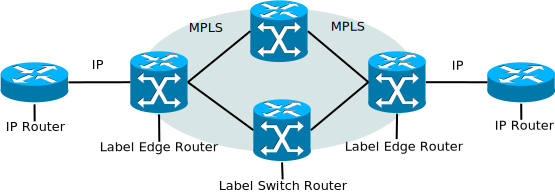
\includegraphics[width=0.9\textwidth]{img/mpls_net}
  \caption[MPLS network]{Example of an MPLS network showing IP
    routers, Label Edge Routers and Label Switching Routers. Traffic
    between the IP and Edge routers is forwarded based on the IP
    header, while within the MPLS network packets are switched on
    labels.}
  \label{fig:mpls_net}
\end{figure}

\newpage

It is also possible to tunnel an LSP inside another LSP, by adding
additional shim headers to the packet; the set of the shim headers
associated to a packet is then called label stack. When the packet is
being forwarded, only the topmost label of the stack is taken into
consideration by the routers and the last label has a special field to
indicate the bottom of the stack. \\
This technique provides great benefits to the scalability of the
network, since it consistently reduces the number of LSPs that have to
be setup and maintained by the routers.

\subsection{Traffic Engineering}
The evolution of the IP technology has allowed traditional IP routing
to catch up and be able to manage efficiently the current speed of the
networks, therefore weakening the initial impulse for the creation of
MPLS\@. Although, MPLS has proved to be particularly suited for the
management of networks using Traffic Engineering.

Traffic engineering may be a familiar concept to civil engineers,
since it was first applied to road traffic, studying how to increase
safety and performance in the transportation system; the analogy
stands strong if we imagine packets as cars, links as roads and
switches and routers as crossroads: the goal of both types of traffic
engineer is to minimize the number of collisions while improving the
traffic flow. How is that done? The various techniques involve
dynamical analysis, predictions and regulation of the behavior of data
transmitted over that network.

In the majority of IP networks, the algorithms used for calculating a
path between two nodes are based on Open Shortest Path First (OSPF):
therefore the shortest path between the nodes is chosen as the best
path; this kind of behavior is logical if we suppose that the network
is unused or lightly used. But what happens when the network is under
heavy usage? In Figure~\ref{fig:mpls_te} Alice is the default gateway
of LAN A and Bob is the default gateway of LAN B; when the traffic
between the two LANs is light, the default path is the shortest and
most efficient solution. Although, the more intense becomes the
traffic between the LANs, the more congested will become the default
path, even if there are clearly two unused paths available.

\begin{figure}[!hbp]
  \centering
  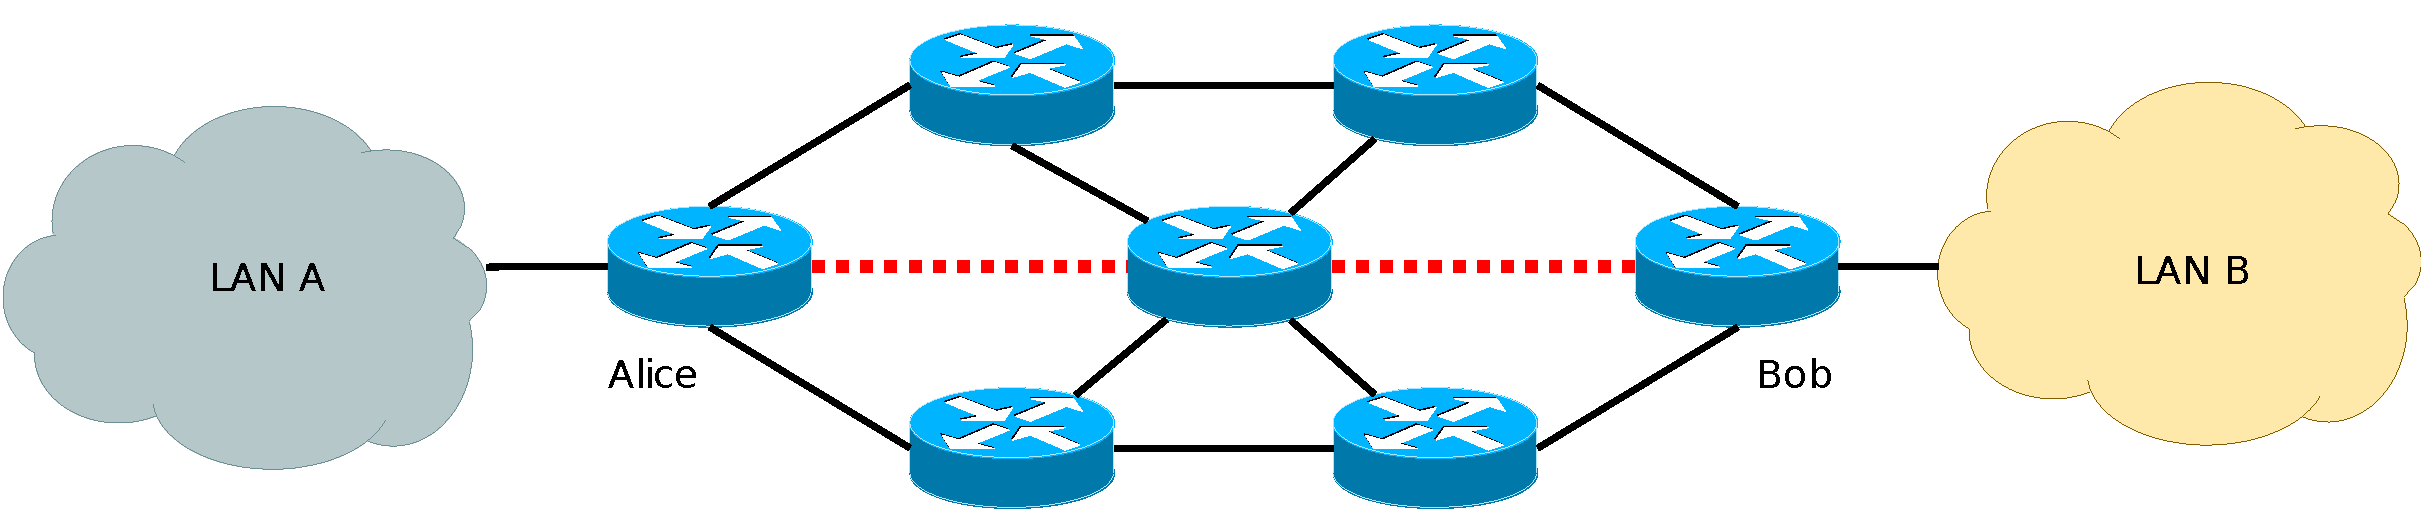
\includegraphics[width=0.9\textwidth]{img/mpls_te}
  \caption[Traffic Engineering]{The more the traffic between LAN A and
    LAN B increases, the more the dotted line becomes congested.}
  \label{fig:mpls_te}
\end{figure}

Traffic Engineering naturally strives to solve this kind of problems
and ensure a better usage of the network resources. To be able to
fulfill this task it is necessary to first build a more complex model
and gain an advanced knowledge of the network architecture; then, this
information has to be used to somehow control the behavior of the
network. MPLS was therefore extended to carry more information about
the network characteristics and allow a much finer degree of
configuration; these extension to the MPLS protocol supporting Traffic
Engineering mechanisms have taken the name of MPLS-TE.

MPLS-TE aims to improve the performance of the network for different
targets: it can assure a certain QOS to a group of streams, for
example minimizing the end-to-end delay or the packet loss rate; this
optimization is particularly evident to the network users, since it
improves dramatically the quality of some applications. On the other
hand, MPLS-TE could also be used by network administrators to ensure
that no network resource is over-utilized or under-utilized, thus
guaranteeing an optimal use of the deployed network devices.

\section{Generalized MPLS}

The traditional way of designing and configuring a network requires
manual interventions: it could take a long time to add a new service
or remove an old one because of the interactions between the various
elements inside the network; when the size and the complexity of the
network increase, this problem gets even harder. This brings up the
need of a control system that is able to automatically configure and
control the service provisioning.

\subsection{Switching Types}

The great innovation of GMPLS is the ability to seamlessly switch many
different network technologies: packet frames, TDM time-slots, fibers
or wavelengths are all treated in the same way. This abstraction makes
the provisioning of services much more efficient and simplifies
enormously the setup of end-to-end connections over network segments
composed by different types of link-layer technology. The GMPLS
protocol defines a set of switchable quantities, called Switching
Types, that are diversified based on the transport layer technology
involved: for example, MPLS routers are defined as \textit{packet
  switch capable (PSC)}, since they are able to recognize and switch
single packets. Ethernet switches are simply \textit{Layer 2 switch
  capable (L2SC)} and Time Division Multiplexing switches are called
\textit{TDM Capable}. Moving on to the optical devices, there is a
distinction between the devices that switch data based on the
wavelength on which the data is received (\textit{Lambda Switch
  Capable (LSC)} and the ones that forward it based on which actual
fiber carried the information (\textit{Fiber Switch Capable (FSC)}.

Although we have classified these network devices based on the
quantities they are able to switch, a clarification needs to be made
in order to better understand the GMPLS architecture: since there are
usually many types of link layer technology involved in this kind of
network, it is not particularly correct to define which quantity a
device can switch, because a device could switch more than
one. Therefore, it would be better to clarify which specific interface
is capable of switching a certain quantity: this is done by a special
descriptor called \textit{Interface Switching Capability Descriptor}
(ISCD).

\begin{figure}[!hbp]
  \begin{center}
    \begin{tabular}{|l|l|l|}
      \hline
      Description & Abbreviation & Value \\ \hline
      Packet-Switch Capable-1 & PSC-1 & 1 \\
      Packet-Switch Capable-2 & PSC-2 & 2 \\
      Packet-Switch Capable-3 & PSC-3 & 3 \\
      Packet-Switch Capable-4 & PSC-4 & 4 \\
      Layer-2 Switch Capable & L2SC & 51 \\
      Time-Division-Multiplex Capable & TDM & 100 \\
      Lambda-Switch Capable & LSC & 150 \\
      Fiber-Switch Capable & FSC & 200 \\
      \hline
    \end{tabular}
    \caption[Interface Switching Capability Descriptor]{The possible
      values of the Switching Capability field in the Interface
      Switching Capability Descriptor as defined by RFC4205.}
    \label{fig:gmpls_iscd}
  \end{center}
\end{figure}

\subsection{Still Label Switching}
The essential feature of MPLS has obviously still a great importance
in GMPLS, even though there are some differences: while in MPLS the
label is assigned to a packet in a rather unpredictable and arbitrary
way and has no logical bound with the contents of the packet, this is
not the case of GMPLS\@. In fact, if we think about \textit{what} is
being switched in a GMPLS network, we can quickly realize that every
switchable data stream also represents a precise physical
resource. For example, in an optical cross-connect a label identifies
a specific wavelength, in a TDM system the label is associated to a
specific time-slot and in a fiber switch the label is directly linked
to a specific port or fiber.

Therefore, in GMPLS the label has an actual meaning and is directly
connected to some physical property of the network. This brings some
other consequences: first of all, it is likely that the label will
belong to a much smaller set of values, for example the available
wavelengths in an optical network segment. Another implication is that
the label needs to be carefully analyzed and interpreted: since its
content represents now an actual resource, it needs to be correctly
understood by any router involved in the process.

\begin{figure}[!tbp]
  \begin{center}
    \begin{bytefield}{32}
      \bitheader{0,7,15,23,31} \\
      \bitbox{32}{Generalized Label}
    \end{bytefield}
    \caption[GMPLS label]{The GMPLS 32-bit Generalized Label.}
    \label{fig:gmpls_label}
  \end{center}
\end{figure}

Given this description of what a label should be, we can understand
how a Label Switched Path (LSP) works: every router in the path is a
cross-connected device, which means that is programmed to receive data
from a certain resource and forward it to another.

Every resource is associated to a label that explains its
characteristics: the LSP consists of a series of triplets
\textit{\{device, interface, label\}} that represents a sequence of
cross-connected devices able to deliver traffic. Then, it can ensure a
full or a partial connectivity supporting a wide range or services and
applications.

The main innovation of the GMPLS LSP is the introduction of
bidirectional paths: when in MPLS we had to setup two different
unidirectional paths, in GMPLS we can use a single bidirectional
path. This has some technical advantages: it requires less memory and
it can be setup more quickly and with lesser signaling
effort. Furthermore, it simplifies considerably traffic engineering
problems regarding error recovery and \textit{fate sharing}.


\subsection{Control and Data Planes}

In packet switching networks, the control plane and the data plane can
be delivered using the same link: for example, in IP routing the
information about the destination of the packet is carried with the
packet itself. In these cases, the control plane and the data plane
can be actually considered coincident. In transport networks though,
the devices are not able to recognize single packets and they switch
entire time-slots, fibers or wavelengths; therefore, the control
information about the data cannot be transmitted using the same medium
(in-band control).

The control plane in GMPLS is generally referred to as the Multi-Layer
Control Plane (MLCP) and is completely separated from the data plane;
it controls the operations of GMPLS network out-of-band. \\
This approach means that a failure on the control plane will not
affect the data plane and vice versa. This separation adds also a
layer of abstraction between the control and the data plane, thus
making possible the interaction between many different data plane
technologies.

In order to traffic engineer the behavior of the network, MLCP uses
routing and signaling protocols based on the IP models: most of the IP
protocols have been extended to support GMPLS; IPv4 or IPv6 addresses
are used to identify interfaces. This also applies in a certain
measure to the data plane, even though \textit{unnumbered links}
(i.e.\ links without an IP address) are also supported when IP
addresses are not available. This is particularly important when the
network is composed by optical devices which do not support the
traditional IP addressing.

\begin{figure}[!htbp]
  \centering
  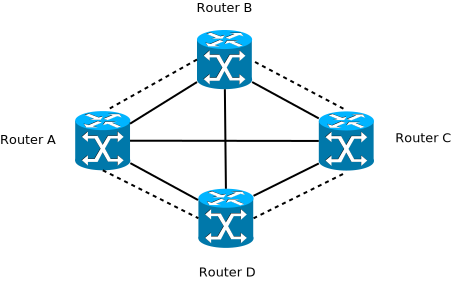
\includegraphics[width=0.75\textwidth]{img/gmpls_mlcp}
  \caption[MPLS network]{The dotted lines represent the control plane
    links, while the normal lines represent the data plane links.}
  \label{fig:gmpls_mlcp}
\end{figure}

There are three different models that the MLCP can be based on: the
peer model, the overlay model and the augmented model. In the peer
model, all the nodes in the network have complete knowledge and
visibility of the other nodes in the network; in the overlay model
instead, all the network layers are clearly separated and the nodes
can only interact directly with the other nodes in the same layer. The
augmented model is a kind of hybrid between the two previous models,
allowing a certain level of peer communication, for example regarding
routing and signaling information but not the entire network
topology. These different models give to MLCP a great flexibility when
dealing with different types of networks.

\subsection{Tunnels and Hierarchies}

The technique used by MPLS to establish tunnels within a network was
\textit{label stacking}, i.e.\ adding more labels to a packet and
letting the MPLS routers analyze only the topmost one; although this
approach works in a network where packets, frames or cells are
switched, it doesn't with the network model proposed by GMPLS, since
some of the network technologies involved do not support stacking: for
example, it is not possible to encapsulate a wavelength inside another
wavelength and extract it back at the end of the tunnel. This is also
related to the fact that in GMPLS the label is logically associated
with the physical resource and to change the label would mean to
modify in some way the physical resource.

Therefore, the meaning of LSP tunnel changes completely in GMPLS: the
hierarchy of the tunnels is now based on the natural difference in
granularity of the different network technologies. This means that the
LSP tunnels follow the same hierarchy of the physical architecture:
packet may be nested in a time-slot, time-slots may be grouped in a
wavelength and wavelengths may be nested in a fiber (as shown in
Figure~\ref{fig:gmpls_hierarchy}).

This solution offers a better scalability to the system, allowing the
aggregation of multiple LSP tunnels and offering the possibility of a
more efficient traffic engineering.

\begin{figure}[!htbp]
  \centering
  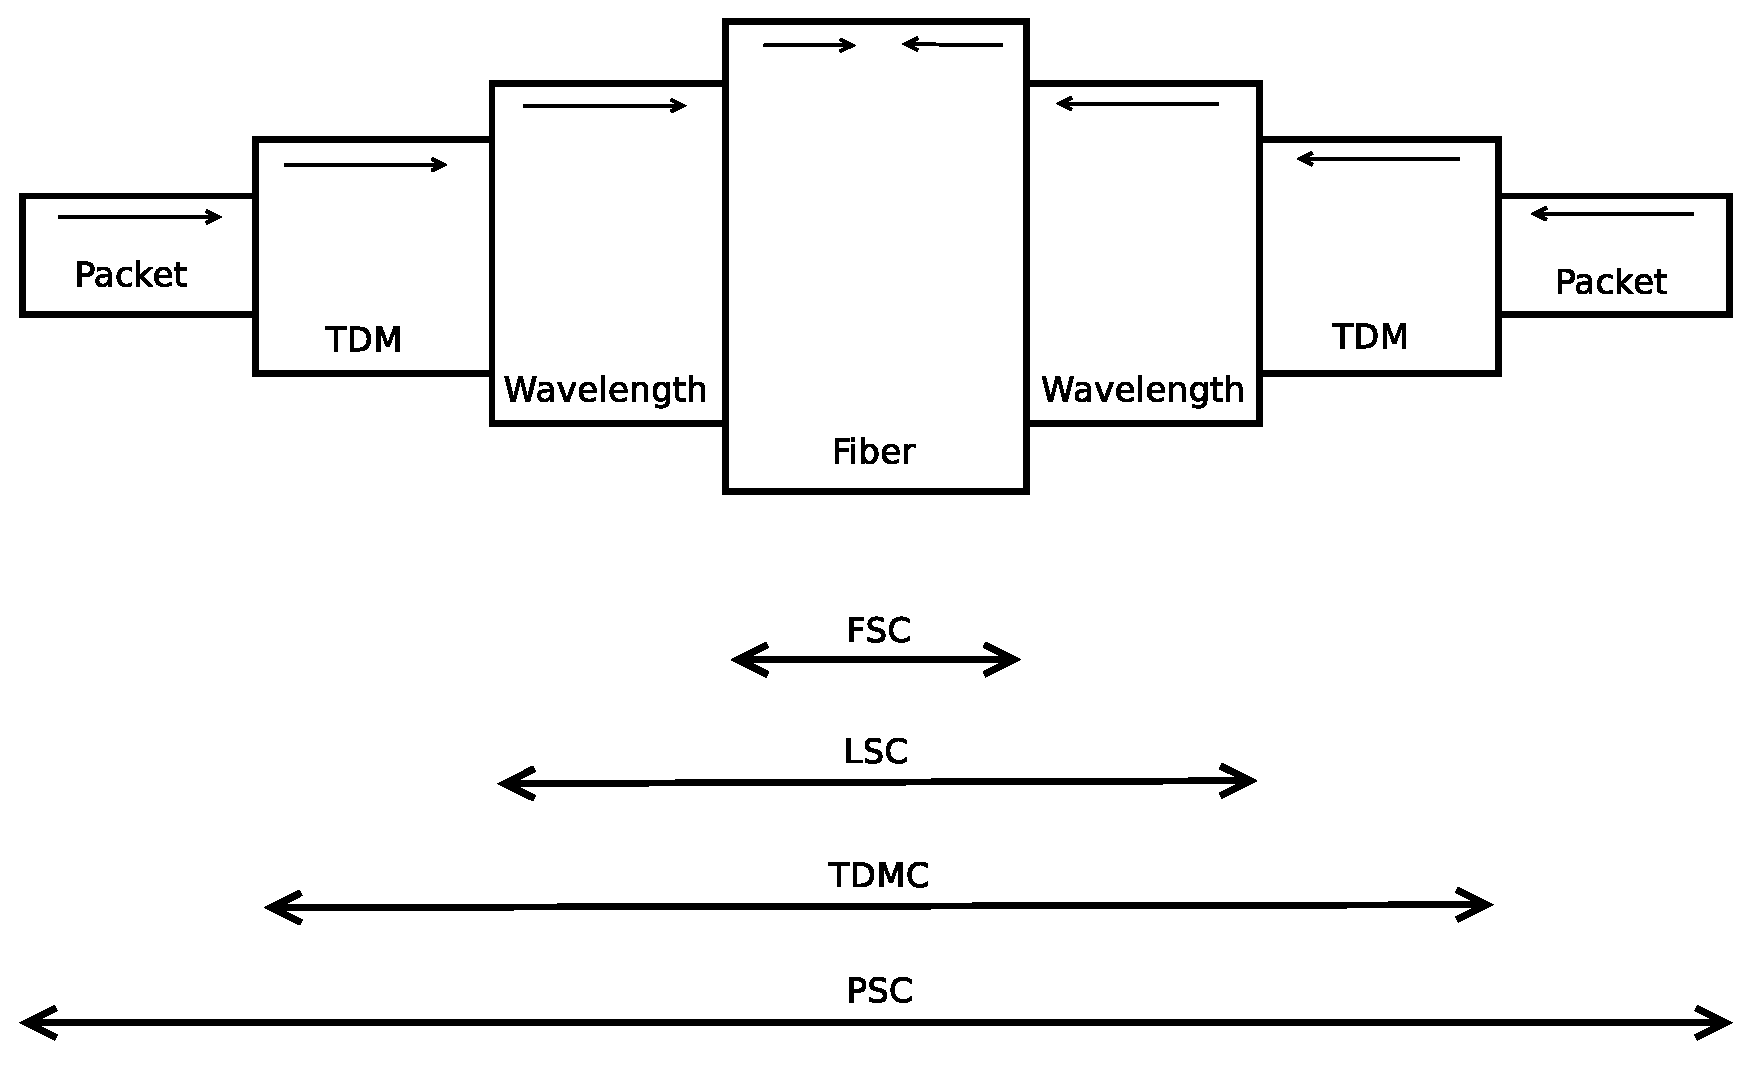
\includegraphics[width=0.9\textwidth]{img/gmpls_hierarchy}
  \caption[GMPLS LSP Hierarchy]{The GMPLS LSP Hierarchy: packets are
    nested in time-slots, which are nested in wavelengths, which are
    nested in fibers.}
  \label{fig:gmpls_hierarchy}
\end{figure}

\subsection{GMPLS Protocols}

In order to make this architecture efficient, a wide range of
protocols has been extended or invented to support GMPLS: these
protocols are used for the routing, the signaling and the link
management of a GMPLS network.

The routing protocols have the task to manage information about the
topology of the network, distributing it across the network: these
protocols are essential for the routing algorithms. The ones currently
available in GMPLS are Open Shortest Path First with Traffic
Engineering additions (OSPF-TE) and Intermediate System to
Intermediate System (IS-IS). OSPF-TE will be taken into consideration.

The signaling consists of the process of establishing and removing
Label Switched Paths: they are very important for service provisioning
since they manage the reservation of the network resources and the
guarantee of a specific Quality of Service. The protocols in use are
Resource ReserVation Protocol with TE additions (RSVP-TE) and
Constraint-based Routing-Label Distribution Protocol (CR-LDP). There
will be an overview of RSVP-TE in the following sections.

Regarding link management, these protocols are used by in a GMPLS
network to discover and verify the connectivity of the links; a new
protocol called Link Management Protocol (LMP) has been introduced to
check the validity of the link advertisements that are exchanged
across the network. LMP will be explained briefly.

\subsection{OSPF-TE}

Open Shortest Path First (OSPF) is an Interior Gateway Protocol (IGP)
and, more specifically, a link-state routing protocol: this means that
it was designed to work within an Autonomous System (AS) by exchanging
information about the link-state configuration of each router. Special
routers called Autonomous System Boundary Routers (ASBR) distribute
inside the network information coming from other Autonomous Systems.

To handle the traffic more efficiently and increase the scalability of
the architecture the AS is divided into several areas: these areas are
connected by routers called Area Border Routers (ABR) which have the
task to propagate the information of their own area to other areas and
receive information from other areas. Inside an Autonomous System
there is a primary area called the \textit{backbone}: all other areas
must be connected to the backbone and the routers inside the backbone
area are called backbone routers.

There are five types of messages that the routers can exchange in
OSPF: Hello, Database Description, Link State Request, Link State
Update, and Link State Acknowledge. They all share the same OSPF
header and are briefly described in Figure~\ref{fig:ospf_messages}.

Basically, each router at first exchange Hello messages with their
neighbours to establish routing adjacency; then, they synchronize
their link databases by exchanging link database descriptors: these
messages contain at least one database data structure, known as Link
State Advertisement (LSA). There are also several types of LSA which
are explained in Figure~\ref{fig:ospf_lsa}. When the database
descriptors of all the routers have been distributed across the
network, the Link State Database can be built and used to calculate
the Shortest Path First routing tables.

\begin{figure}[!tbp]
  \begin{center}
    \begin{tabular}{|l|l|p{0.45\textwidth}|}
      \hline
      Type & Name & Description \\ \hline
      1 & Hello & Used to discover neighbours and maintain routing
      adjacency. \\
      2 & Database Description & List the available link state
      information without actually supplying it. \\
      3 & Link State Request & Request information regarding the link
      state configuration. \\
      4 & Link State Update & Primary message in OSPF-TE: used to
      distribute link state information. \\
      5 & Link State Acknowledgement & Acknowledges the reception of
      link state messages. \\
      \hline
    \end{tabular}
    \caption[OSPF Messages]{The various types of message in OSPF}
    \label{fig:ospf_messages}
  \end{center}
\end{figure}

One of the most important elements for GMPLS routing is the ``Link
State Update'' message, because it carries along one or more LSAs and
it is exchanged between adjacent routers at specific intervals. For
Traffic Engineering purposes, a special type of LSA is introduced: to
make it invisible to the normal OSPF routing, this LSA is made
\textit{opaque}; this LSA will be ignored by every router but the ones
involved in the GMPLS routing process.

\newpage

This opaque LSA has the standard LSA header followed by a Type Length
Value (TLV) field: usually this TLV is composed by a list of sub-TLVs
which contains the actual Traffic Engineering information, such as the
router ID, the local and the remote IP addresses, the reserved
bandwidth, the reservable bandwidth etc.

\begin{figure}[!tbp]
  \begin{center}
    \begin{tabular}{|l|l|p{0.60\textwidth}|}
      \hline
      Type& Name & Description \\ \hline
      1 &  Router & Sent from a router to other routers in the same
      area; it contains information about the router interfaces, IPs
      and its adjacent routers. \\
      2 & Network & Generated by the gateway of the network segment;
      it contains information about the whole segment. \\
      3 & Network Summary & Generated by ABRs and contains a summary
      of the network area; it is used to inform the neighbour areas. \\
      4 & ASBR Summary &  Generated by ASBRs and contains all the
      information about the internal structure of an AS \\
      5 & AS external &  This LSA contains information brought by
      External Gateway Protocols, regarding other ASs. \\
      9 & Link-local Opaque & This LSA is used for TE purposes: it
      carries opaque information within a network. \\
      10 & Area-local Opaque & This LSA is also used for TE purposes:
      it carries opaque information within an area. \\
      11 & External Opaque & Another LSA used for TE purposes: it
      carries opaque information within an AS. \\
      \hline
    \end{tabular}
    \caption[OSPF-TE LSA Types]{OSPF-TE LSA types, names and
      descriptions}
    \label{fig:ospf_lsa}
  \end{center}
\end{figure}

The TE information will be then used to create a new type of Database,
called the Traffic Engineering Database (TED); the TED has a critical
importance in the TE routing mechanisms, since it is the main source
of information for the Constrained Shortest Path First (CSPF)
algorithms that are employed in this context. Using the TED a new
model of the network that takes in account TE variables can be built,
while CSPF algorithms compute network paths between nodes in the
network. In the next chapter, this type of algorithm will be
thoroughly reviewed and explained.

\subsection{RSVP-TE}

RSVP-TE the signaling protocol used in GMPLS to establish, maintain,
modify and destroy paths in the data plane. This protocol is composed
by a wide range of messages that are exchanged among the various nodes
involved in the network: these messages need to respect a precise set
of rules enforced by the so-called \textit{signaling controllers},
which are the software components responsible for the management of
the data plane behaviour of the Label Switching Routers.

The establishment of a Label Switched Path is generally initiated by
the ingress LSR (logically intended as the \textit{upstream} end of
the LSP), which sends a \textit{LSP Setup} message. The
\textit{downstream} LSR receives this message and replies with a
\textit{LSP Accept} message; the confirmation of the establishment of
the LSP may be signaled using the \textit{LSP Confirm} message. If any
error should happen during the setup, they can be signaled either
downstream or upstream using the \textit{LSP Downstream Error} or the
\textit{LSP Upstream Error} messages. Any router that form the LSP can
initiate the tear down by sending \textit{LSP Downstream Release} or
\textit{LSP Upstream Release} messages. In order to distribute the
information concerning the state of the data plane, \textit{LSP
  Notify} messages are used. In Figure~\ref{fig:rsvp_messages} we can
see a mapping between these abstract messages and the ones utilized in
RSVP-TE.

\begin{figure}[!htbp]
  \begin{center}
    \begin{tabular}{|l|l|}
      \hline
      Abstract Message &  RSVP-TE Message \\ \hline
      LSP Setup & Path \\
      LSP Accept & Resv \\
      LSP Confirm & Resv-Confirm \\
      LSP Upstream Error & PathErr \\
      LSP Downstream Error & ResvErr \\
      LSP Downstream Release & PathTear \\
      LSP Upstream Release & PathErr \\
      LSP Notify & Notify \\
      \hline
    \end{tabular}
    \caption[RSVP-TE Messages]{The various types of message in
      RSVP-TE}
    \label{fig:rsvp_messages}
  \end{center}
\end{figure}

The signaling message is generally composed by multiple signaling
objects that share a common header: when a LSP receives one of these
messages the header is first extracted to identify the type of the
objects; then, each object is separately analyzed and processed. The
task of generalizing RSVP boiled down to the task of creating new
signaling objects and adding some improvements to the signaling
protocol like rapid notification and bidirectional LSPs.

\begin{figure}[!htbp]
  \centering
  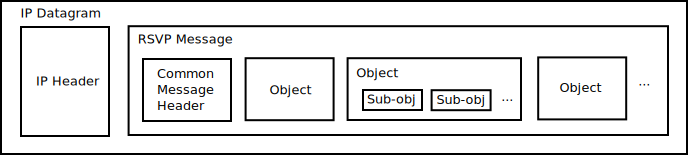
\includegraphics[width=0.9\textwidth]{img/rsvp_message}
  \caption[RSVP Message]{A RSVP Message, included in a IP data-gram
    and composed by multiple objects; each of the objects may be
    composed by multiple sub-objects.}
  \label{fig:rsvp_message}
\end{figure}

The \textit{Common Message Header} is generally a 8-byte field and
identifies the message; the encapsulated objects are instead of
variable length and are structured as type-length-value triplets. This
structure makes parsing much easier and provides a more flexible
configuration. In the same way, each object may incorporate multiple
sub-objects, which are encoded as TLV constructs as
well. Figure~\ref{fig:rsvp_message} shows how a GMPLS RSVP-TE message
composed by objects and sub-objects is encapsulated inside a IP
packet.

\subsubsection{LSP Establishment}
One of the main improvements of RSVP-TE over RSVP is the possibility
of creating bidirectional paths: this requires a full set of Path and
Resv messages to be exchanged between two LSRs. The ingress LSR sends
a \textit{Path} message downstream to the next router initiating the
creation of the LSP\@. This \textit{Path} message contains the
Upstream Label, i.e.\ the label to be used in the upstream direction,
various information about the path and a Generalized Label Request
object, needed for the LSP setup request.

If the Path message is delivered correctly to the next hop, the
upstream label is saved and a path state is reserved to guarantee the
correct handling of the next messages. This router then proceeds to
replace the upstream label with its own, create a state for the
upstream direction and forwarding the Path message to the next
router. This process continues for each node in the path until the
message reaches the egress LSR; when that happens, the LSP has been
successfully established in the upstream direction, but not yet in the
downstream one (i.e.\ the label distribution is downstream-on-demand,
which means that upstream LSRs request downstream LSRs to choose the
labels). Therefore, the egress LSR creates a \textit{Resv} message,
similar to the Path message except that it contains a Generalized
Label object instead: this object contains a downstream label. The
Resv message is then forwarded back along the same path: each router
receiving the Resv message save the state for the downstream
direction, replaces the label and forward it. When the ingress LSP
receives the Resv message, the LSP has been successfully setup in both
upstream and downstream directions. Figure~\ref{fig:rsvp_path} shows
an example of this process.

\begin{figure}[!htbp]
  \centering
  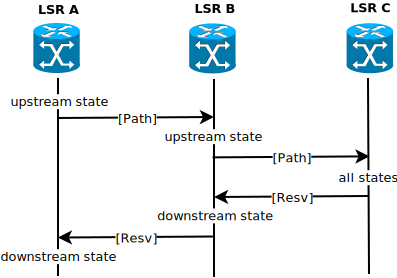
\includegraphics[width=0.7\textwidth]{img/rsvp_path}
  \caption[RSVP-TE path setup]{RSVP-TE bidirectional path setup with
    messages and states.}
  \label{fig:rsvp_path}
\end{figure}

\subsubsection{LSP removal}

There are two types of message used in RSVP-TE to remove LSPs,
\textit{PathTear} and \textit{PathErr}; when a LSR decides to remove a
path, it sends a PathTear message following the direction of a Path
message and a PathErr message following the direction of a Resv
message. Each router that receives these messages clear their states
and forward them along the path, allowing a fast and reliable release
of the LSP; both downstream and upstream directions can be cleared
simultaneously. Additionally, using the \textit{Notify} message, any
router can signal to the ingress or the egress LSR eventual errors and
malfunctions and ask them to initiate the LSP removal (\textit{Rapid
  Error Notification}). Basically, these two different mechanisms can
be used alternatively to remove an LSP (shown in
Figure~\ref{fig:rsvp_tear}): while the Notify approach is more
classic, the PathTear/PathErr one increases considerably the signaling
efficiency.

\begin{figure}[!htbp]
  \centering
  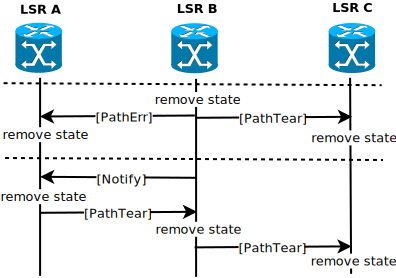
\includegraphics[width=0.7\textwidth]{img/rsvp_tear}
  \caption[RSVP-TE path removal]{The two mechanisms included in GMPLS
    to remove LSPs.}
  \label{fig:rsvp_tear}
\end{figure}

\subsubsection{Error handling}

During the whole process of establishing and removing LSPs across our
network, we can easily guess that sooner or later errors are going to
occur: to manage this kind of situation, RSVP-TE includes two types of
error messages, \textit{PathErr} and \textit{ResvErr}. The PathErr
message indicates a malfunction of the Path message and is sent
towards the ingress LSR, while the ResvErr message is used to signal
an error during the forwarding of the Resv message and is sent towards
the egress LSR\@. When a router receives these messages, it can either
try to solve the problem by itself or forward it along.

\subsubsection{Explicit Route Object}

The Explicit Route Object (ERO) is one of the objects added to RSVP in
order to manage traffic engineering problems: this object basically
contains the list of the abstract nodes that have to be visited by the
LSP\@. Each abstract node can be either IPv4, IPv6 or an Autonomous
System. Another important distinction is if the node is ``strict'' or
``loose'', which mostly influences the path between the current node
and the previous node: if a node is strict, the path followed to reach
it must be part of the previous abstract node; if a node is loose, the
path followed to reach it could also traverse nodes that aren't part
of the previous abstract node.

\begin{figure}[!htbp]
  \begin{center}
    \begin{bytefield}{16}
      \bitheader{0,1,7,8,15} \\
      \bitbox{1}{L} \bitbox{7}{Type}
      \bitbox{8}{Length} \\
      \bitbox{16}{IPv4 Address} \\
      \bitbox{16}{IPv4 Address (Cont.)} \\
      \bitbox{8}{Prefix Length}
      \bitbox{8}{Reserved} \\
    \end{bytefield}
    \caption[Explicit Route Object]{An example of IPv4 ERO sub-object:
      the header is composed by the L flag which specifies if the hop
      is strict or loose, the Type field which specifies if the
      sub-object is IPv4, IPv6 or and AS and the Length field. The
      actual sub-object contains an IPv4 address, a prefix length
      (netmask) and reserved bits.}
    \label{fig:ero_ipv4}
  \end{center}
\end{figure}

The ERO is included in the Path or Resv messages that are exchanged
during the installation of the LSP: while the Path message is
forwarded along the path, each node listed in the ERO is subsequently
removed. When the Path message reaches the egress LSR, the ERO list is
therefore empty and there is no other information of which path the
message has followed except for the previous hop: to be able to
recover this information, the list of abstract nodes traversed is
copied in the Record Route Object (RRO). The egress router may read
this object to know the exact path and eventually share it with the
ingress router in a Resv message.

\begin{figure}[!htbp]
  \begin{center}
    \begin{bytefield}{32}
      \bitheader{0,8,16,24,32} \\
      \bitbox{1}{L} \bitbox{7}{Type} \bitbox{8}{Length} \bitbox{1}{U}
      \bitbox{7}{Reserved (0)}
      \bitbox{8}{Class Type (2)} \\
      \bitbox{32}{Generalized Label} \\
    \end{bytefield}
    \caption[Label ERO sub-object]{The Label ERO sub-object.}
    \label{fig:ero_label}
  \end{center}
\end{figure}

The ERO signaling object has also been extended to support explicit
label control: a label ERO sub-object has been added which specifies
which labels have to be installed on the interfaces of a node. The
label ERO sub-objects (both downstream and upstream may be specified)
are added next to the already existing ERO sub-objects. This method
makes a lot easier to distribute the GMPLS generalized labels and is,
in fact, the default method utilized in GMPLS for setting up a LSP.

\subsection{LMP}

The \textit{Link Management Protocol} has been designed to overcome
the structural complexity of GMPLS networks: since many different data
layers are possible and that the data plane and the control plane are
sometimes physically separate, it is not that straightforward for two
neighbours to refer to each data channel in an unambiguous way that
the other node will certainly understand. The task of LMP is to help
these nodes to discover the characteristics and the identifiers of the
links to which they are connected; moreover, this protocol has proved
to be extremely useful to monitor the network, detect failures and
isolate them. The main features of LMP, described in RFC4204, are:
\begin{itemize}
\item \textbf{Link correlation} \\
  Data links are aggregated into TE links and data links features are
  exchanged in order to perform consistency checks.
\item \textbf{Link verification} \\
  Data links connectivity is analyzed in order to dynamically discover
  TE capabilities and data link remote id.
\item \textbf{Fault localization} \\
  This feature allows to determine exactly where the failure has
  happened, isolating it between a node and its adjacent downstream
  node.
\item \textbf{Service discovery} \\
  The exchange of information regarding the client service
  capabilities and the transport network services is enabled.
\item \textbf{Trace monitoring} \\
  This feature allows some nodes to perform trace monitoring, for
  example using SONET/SDH technology.
\end{itemize}

\chapter{GMPLS Path Computation}

This chapter will focus on the concepts on which is based path
computation in GMPLS, starting from the basic definitions; later, it
will proceed to describe the specific architecture and algorithms
involved. Then, it will treat the various constraints that need to be
analyzed.

\section{Basic definitions}

A \textit{transport service} is a system designed to provide a range
of services to the end user by delivering traffic from the information
source to the information destination while ensuring a certain
quality; this quality of service (QOS) is arranged on the base of a
deal between the service provider and the end user. A \textit{path} is
a sequence of network resources of the service provider, which are
able to provide the aforementioned service if provisioned correctly.

\textit{Path computation} can be described as the whole process of
choosing a certain path or a group of paths among the set of possible
alternatives; this process can be done either at the time when the
service is requested (\textit{on-line path computation}) or before any
kind of service is requested (\textit{off-line path
  computation}). While hybrid models support both types of behaviour,
the GMPLS approach tends to prefer on-line computation. Another
important architectural difference is if all paths are computed on the
same node (\textit{centralized path computation}) or if there is a
group of nodes which cooperate to find viable paths
(\textit{distributed path computation}). For the sake of simplicity,
this thesis will only treat the case of a single centralized node.

\section{Path Computation Element}

The Path Computation Element (PCE) is defined by the IETF in RFC4655
as:
\begin{quote}
  \textit{``An entity (component, application, or network node) that
    is capable of computing a network path or route based on a network
    graph and applying computational constraints.''}
\end{quote}
We can see that the definition of PCE is left intentionally abstract:
the PCE might be a software component, program or a network node; it
could even be a complete framework, aware of the network resources and
the multiple constraints involved, which has been specifically
designed for computing complex paths inside the network.

The path computation mechanism is started when a \textit{Path
  Computation Client} (PCC) sends a request to the PCE asking for the
computation of a specific path (similarly to the PCE, also the PCC is
more like an abstract entity rather than a specific device: it can be
a GMPLS router, another PCE, etc.). The PCE calculates the path and
sends it back to the PCC, that will then proceed to signal the new LSP
with a relatively high confidence; although, due to the nature of the
PCC/PCE interaction there aren't any type of guarantees that the LSP
will be setup correctly. Figure~\ref{fig:pce_pcc} shows a model which
represents this interaction.

\begin{figure}[!htbp]
  \centering
  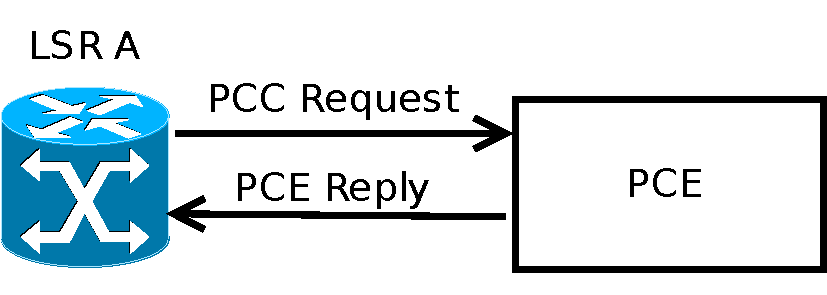
\includegraphics[width=0.5\textwidth]{img/pce_pcc}
  \caption[PCE/PCC Model]{The PCE/PCC interaction model; in this case,
    the PCC is represented by a LSR.}
  \label{fig:pce_pcc}
\end{figure}

\subsection{PCE Architecture}
As we have explained before, in the PCE architecture the
centralized/distributed distinction is very important: multiple PCEs
would certainly distribute the load of the requests, increase the
scalability of the system and solve the annoying
single-point-of-failure problem of the centralized model. On the other
hand, it is unclear if the performance of the distributed model would
actually improve, since the risk of calculating and assigning the same
path increases (\textit{path contention}): this is one of the reasons
that make the PCE reply not certainly assured.

In addition to this difference, the PCE architecture distinguishes
also between the \textit{composite} and the \textit{external} models:
in the composite model, shown in Figure~\ref{fig:pce_composite}, the
PCE functionality is added to a GMPLS router. \\
The signaling engine of this LSR receives the service request and,
acting as PCC, send to the internal PCE a PCC request: the PCE uses
this request to exchange information with the \textit{Traffic
  Engineering Database} (TED), calculates the required path and sends
back a PCE reply to the PCC\@. When this reply is received, the
signaling engine can create a new signaling request and initiate the
LSP establishment.

\begin{figure}[!htbp]
  \centering
  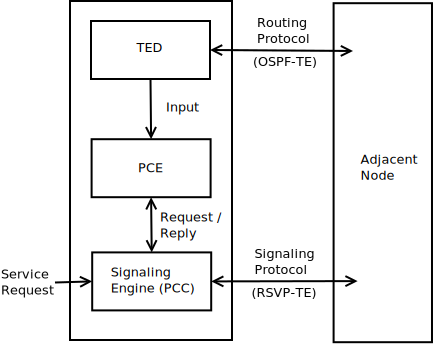
\includegraphics[width=0.6\textwidth]{img/pce_composite}
  \caption[Composite PCE model]{A composite PCE node.}
  \label{fig:pce_composite}
\end{figure}

In the external model, instead of adding the PCE functionality to an
already existing device, a new and independent PCE entity is
introduced; although, the mechanism is very similar to the composite
model: when the head-end node receives the service request, it sends a
path computation request to the PCE, which uses the information in the
TED to compute the path and sends back to the head-end node a
reply. This model is shown in Figure~\ref{fig:pce_external}.

\begin{figure}[!htbp]
  \centering
  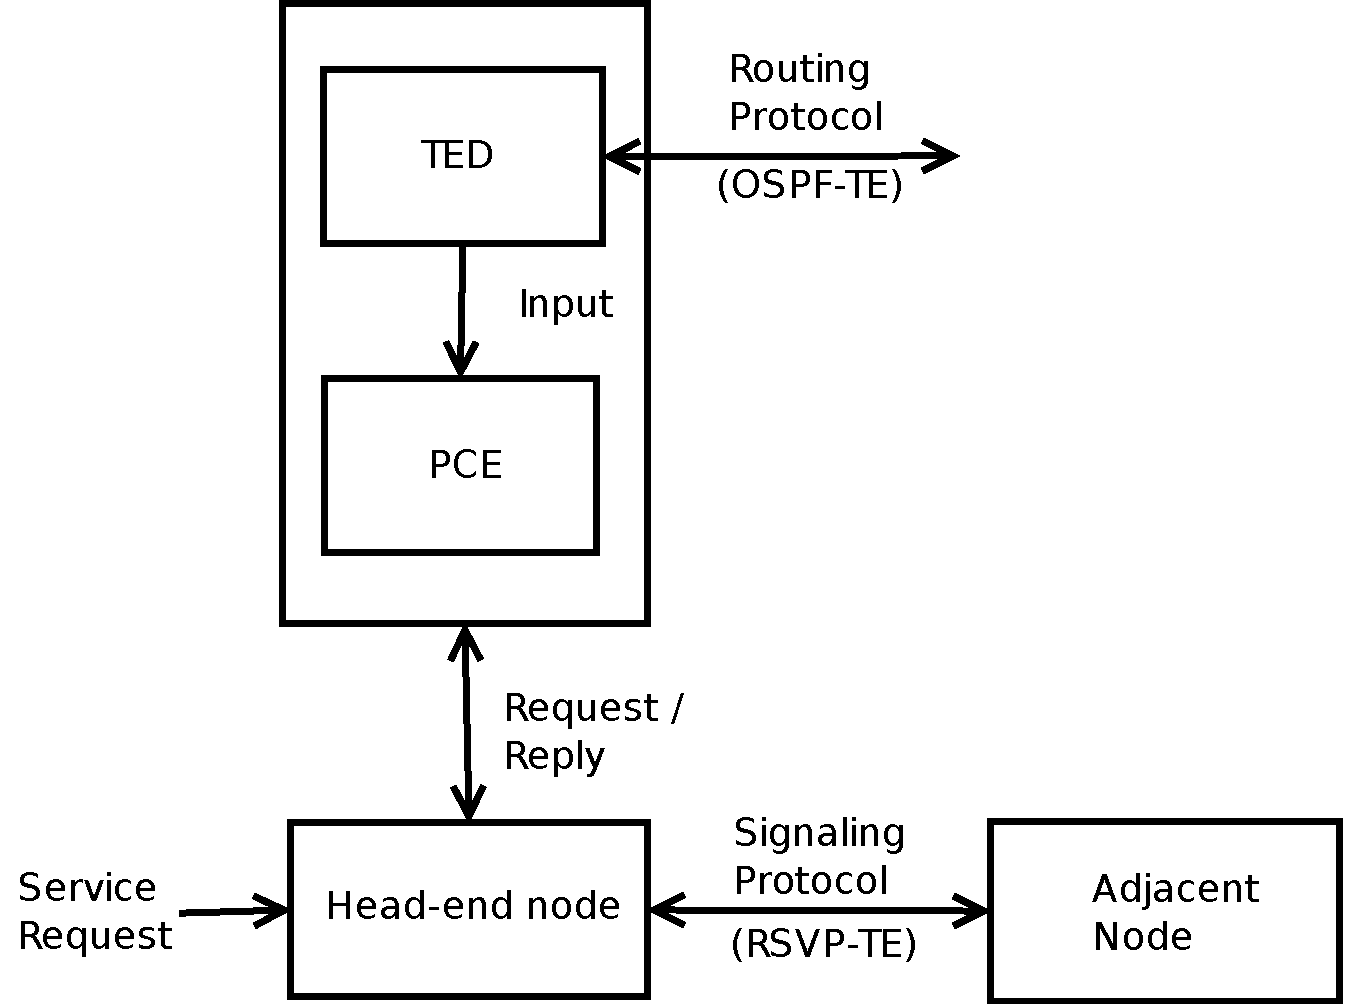
\includegraphics[width=0.65\textwidth]{img/pce_external}
  \caption[External PCE model]{An external PCE node.}
  \label{fig:pce_external}
\end{figure}

If there aren't important logical changes, then why the external PCE
model has been proposed? There are a number of reasons that could
explain why this model was created:
\begin{itemize}
\item Path computation is generally a computationally intensive
  operation and requires a significant amount of resources: even if
  the software is appropriately designed, the stress on the hardware
  can't be underestimated since the PCE component must compute all the
  primary, backup and service paths.
\item Since it requires considerable resources to run, it is more
  likely that the PCE won't be embedded in a regular router, but would
  be deployed in a separate device.
\item Since PCE is designed to provide on-line path computation, the
  response should be quick, in the order of few seconds.
\item The computational power required grows with the size and the
  complexity of the network, i.e.\ multiple constraints like
  bandwidth, latency, cost or QOS to keep in consideration.
\item The main function of a router is the routing process: thus, its
  visibility of the network is limited, its topology knowledge is
  incomplete and it is unfit to perform the complex calculations
  required by a modern multi-layer network.
\item In a very large network, the size of the TED increases very
  quickly: moving the database to a dedicated PCE server would
  decrease the response time of the path requests.
\item If a failure should occur in the network, the PCE could provide
  emergency routing alternatives because of its knowledge of the
  network and its fast response time.
\end{itemize}

As we have seen, the PCE uses the information available in the TED to
compute the requested paths; if the PCE only uses that information,
it's called \textit{stateless}. Instead, a PCE is called
\textit{stateful} if it uses also the information of the
already-computed paths and reserved resources to gain a broader
knowledge of the network status; although this approach allows to
optimize path computation, it also requires a greater effort in terms
of resources and mechanisms to maintain a coherent view of the network
status.

When a client asks the computation of a certain path, the PCE extracts
from the TED the structure and the information regarding the network
in a form of \textit{graph} and applies a certain \textit{path
  computation algorithm} on that representation. This algorithm is
therefore the core of the PCE logic and from its nature depends the
speed, the reliability and the success of the whole PCE.

\section{Constrained Path Computation}

This section will start from the basics of path computation, defining
what is a graph, what is a path and what are the most common path
computation problems. Later it will explain the fundamental algorithms
that have been discovered. The last part will then focus on how to
extend these algorithms to support constrained path computation.

\subsection{Basic definitions}

The most common way to represent a network is to use a \textit{graph}
(an example can be seen in Figure~\ref{fig:graph_example}): the
vertices represent the network nodes and the arcs represent the links;
each arc may also be assigned a number, the \textit{weight}, which
represents the cost of that specific link. If we suppose that the cost
of every link will be the same, we can use weight equal to 1 for every
arc; if we want instead to emphasize the differences between the links
we can also use zero or negative numbers. \\
A \textit{path} is a sequence of adjacent arcs which connects a pair
of vertices: in our example, the nodes A and D are connected by the
paths A-D, A-B-E-D, A-B-E-G-F-C-D, and so on. If a path visits the
same node twice, a \textit{loop} will be formed: the path
A-B-E-G-F-C-A-D contains a loop, since the node A has been visited
twice. If we sum up all the weights of the arcs that form a path, the
total cost of the path will be found; if there are two paths
connecting the same nodes and the first path's cost is lesser than the
other, we'll say that the first path is \textit{shorter}. This may
sound counter-intuitive since we normally associate the length of a
path with the number of arcs that is composed of, but this is only true
when the weight of every arc is 1: in that case, the length of the
path is just the hop count.

\begin{figure}[!hbp]
  \begin{center}
    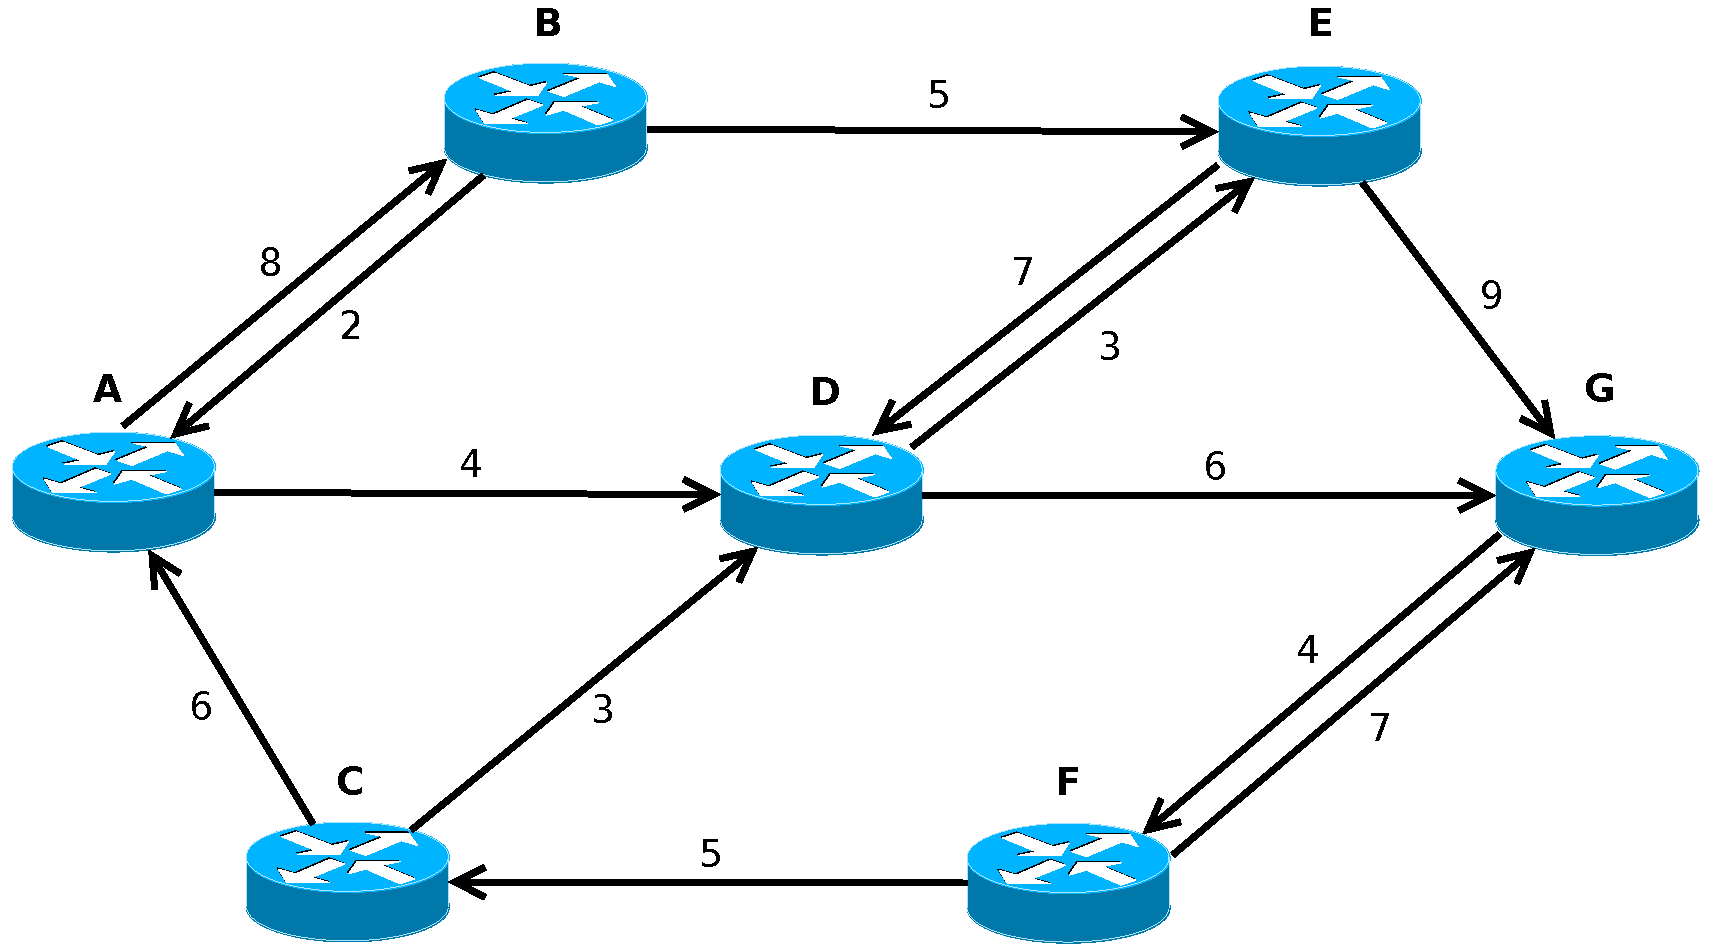
\includegraphics[width=0.8\textwidth]{img/graph_example}
    \caption[Graph example]{A network graph representation with vertices
      as nodes and arcs as links; each arc has a weight, which
      represents the cost of the link.}
    \label{fig:graph_example}
  \end{center}
\end{figure}

What are then the most common path computation problems? Here follows
a short list:
\begin{itemize}
\item \textit{Single-source shortest path}: given a source node, the
  shortest paths to all the other nodes have to be computed.
\item \textit{Single-destination shortest path}: given a destination
  node, the shortest paths from all the other nodes have to be found.
\item \textit{Single-pair shortest path}: give a pair of source node
  and destination node, the shortest path has to be found.
\item \textit{All-pairs shortest path}: given a network, all the
  possible paths between the nodes have to computed.
\end{itemize}

Actually, the solution to the last three problems boils down to solve
the first one: in the single-destination problem, if we invert the
direction of the paths we return to the single-source problem; the
single-pair problem is contained by the single-source and the
all-pairs problem can be obtained by applying the single-source to
every node in the network. Therefore, we will analyze the most
important single-source algorithms.

\subsection{Basic single-source algorithms}

The most important single-source algorithms that will be discussed are
the Bellman-Ford, the Dijkstra, the Modified Dijkstra and the Breadth
First Search algorithms. Even if the specific procedural approach of
these algorithms may differ, they are all based on the same set of
assumptions:
\begin{itemize}
\item \textbf{A shortest path is composed by shortest paths}: if the
  shortest path connecting nodes A and B crosses nodes C and D, then
  it must contain also the shortest path between nodes C and D.
\item \textbf{A shortest path is loop-less}: if a shortest path could
  contain a loop, the same loop could be removed and the cost of the
  loop subtracted to the cost of the path, thus creating a new path
  shorter than the shortest path; therefore, a shortest path should
  not contain loops. 
\item \textbf{Use common variables}: all the aforementioned algorithms
  associate two variables to each vertex v in the graph, the
  \textit{path estimate} d[v] and the \textit{predecessor}
  \(\pi\)[v]. When the computation of the algorithm terminates, the
  path estimate will contain the cost of the shortest path between the
  source node and the v vertex, while the predecessor will contain the
  second-last node that forms the path. In order to build the complete
  path between the source and the node v, it is simply required to
  follow the predecessors' chain, starting from \(\pi[v]\), moving to
  \(\pi[\pi[v]]\), and so on.
\item \textbf{Use common procedures}
\end{itemize}












\chapter{Testing and verification}

In this chapter, the functionality of the whole network that has been
used as testbed will be analyzed; then, we will move to the
verification of the software implementation and an explanation of the
performance results.

\section{Testbed environment}

The testbed environment at Acreo is composed by a variety of network
devices: while some are virtualized through VMware, some are actual
devices. While this allowed to easily create a multi-layer GMPLS
network and grant a good level of flexibility, some of the results
obtained in the testbed may differ from a scenario where all nodes are
real devices: this is caused by the different behaviour of the virtual
interfaces and the high load assigned to the virtual machines. Here is
a list of the physical devices:
\begin{itemize}
\item \textbf{Juniper IP/MPLS routers}: in the network there are three
  Juniper M-series IP/MPLS routers. These device have not been used
  during the testing.
\item \textbf{Linux IP/MPLS routers}: three IP/MPLS routers have been
  implemented patching the Linux kernel for MPLS support; each of
  these routers run on a Dell Dimension 5150 with a 3 GHz processor
  and 512 MB of RAM\@. They are labeled as LR1, LR2 and LR3 in
  Figure~\ref{fig:testbed_model}.
\item \textbf{Switchcore Ethernet switches}: these devices are
  Switchcore Xpeedium2 RD1100 Ethernet switches. Each of these
  switches is controlled via a serial cable by a computer with the
  same specifics of the Linux IP/MPLS routers. These switches are
  called SwCE1, SwCE2 and SwCE3.
\item \textbf{Transmode optical switches}: in the testbed there are
  also three optical switches with several modules, like transponders,
  add-drop multiplexers and cross-connects. These devices were not
  operational during the testing phase.
\end{itemize}

The virtual network is hosted through two different servers, a HP
xw8400 and a Dell Optiplex GX620. Their specifics can be seen in
Figure~\ref{fig:testbed_vm}. All the virtual machines have Ubuntu 6.06
as operative system using the 2.6.15-16 Linux kernel: the HP server
hosts three optical nodes (vROADM1, vROADM2 and vROADM3), an optical
cross-connect (vOXC1) and three Ethernet/Optical boundary devices
(vEC1, vEC2 and vEC3), while the Dell server hosts three Ethernet
switches (vE1, vE2 and vE3).

\begin{figure}[!htbp]
  \begin{center}
    \begin{tabular}{|l|l|l|}
      \hline
      & \textbf{HP xw8400} & \textbf{Dell Optiplex GX62} \\ \hline
      Processor & Intel Xeon 5335 & Intel Dual Core\\ \hline
      Core speed & 2.66 GHz & 3.00 GHz \\ \hline
      RAM & 4 GB & 3 GB \\ \hline
      Disk storage & 1 TB & 250 GB \\ \hline
      Operative System & 32-bit Ubuntu Feisty 7.04 & 32-bit Ubuntu Edgy
      6.10 \\ \hline
      Linux kernel & 2.6.20-16 & 2.6.17-17 \\ \hline
      VMware Server & 1.0.3, build=44356 & 1.0.1, build=29996 \\ \hline
      \multirow{3}{*}{Virtual Machines} & vROADM1, vROADM2 & vE1, vE2,
      vE3 \\
      & vROADM3, vOXC1 & \\
      & vEC1, vEC2, vEC3 & \\ \hline
    \end{tabular}
    \caption[Virtual machines sever specifics]{Hardware and software
      specifics of the servers deploying the virtual machines.}
    \label{fig:testbed_vm}
  \end{center}
\end{figure}

Since some of the network devices weren't functional during the
testing phase, the network representation graph in
Figure~\ref{fig:testbed_model} does not include them; instead, all the
relevant information concerning the data and the control plane are
listed, like nodes and links
identifiers. Figure~\ref{fig:testbed_legend} acts as a reference to
each node in the network.

\begin{figure}[!htbp]
  \begin{center}
    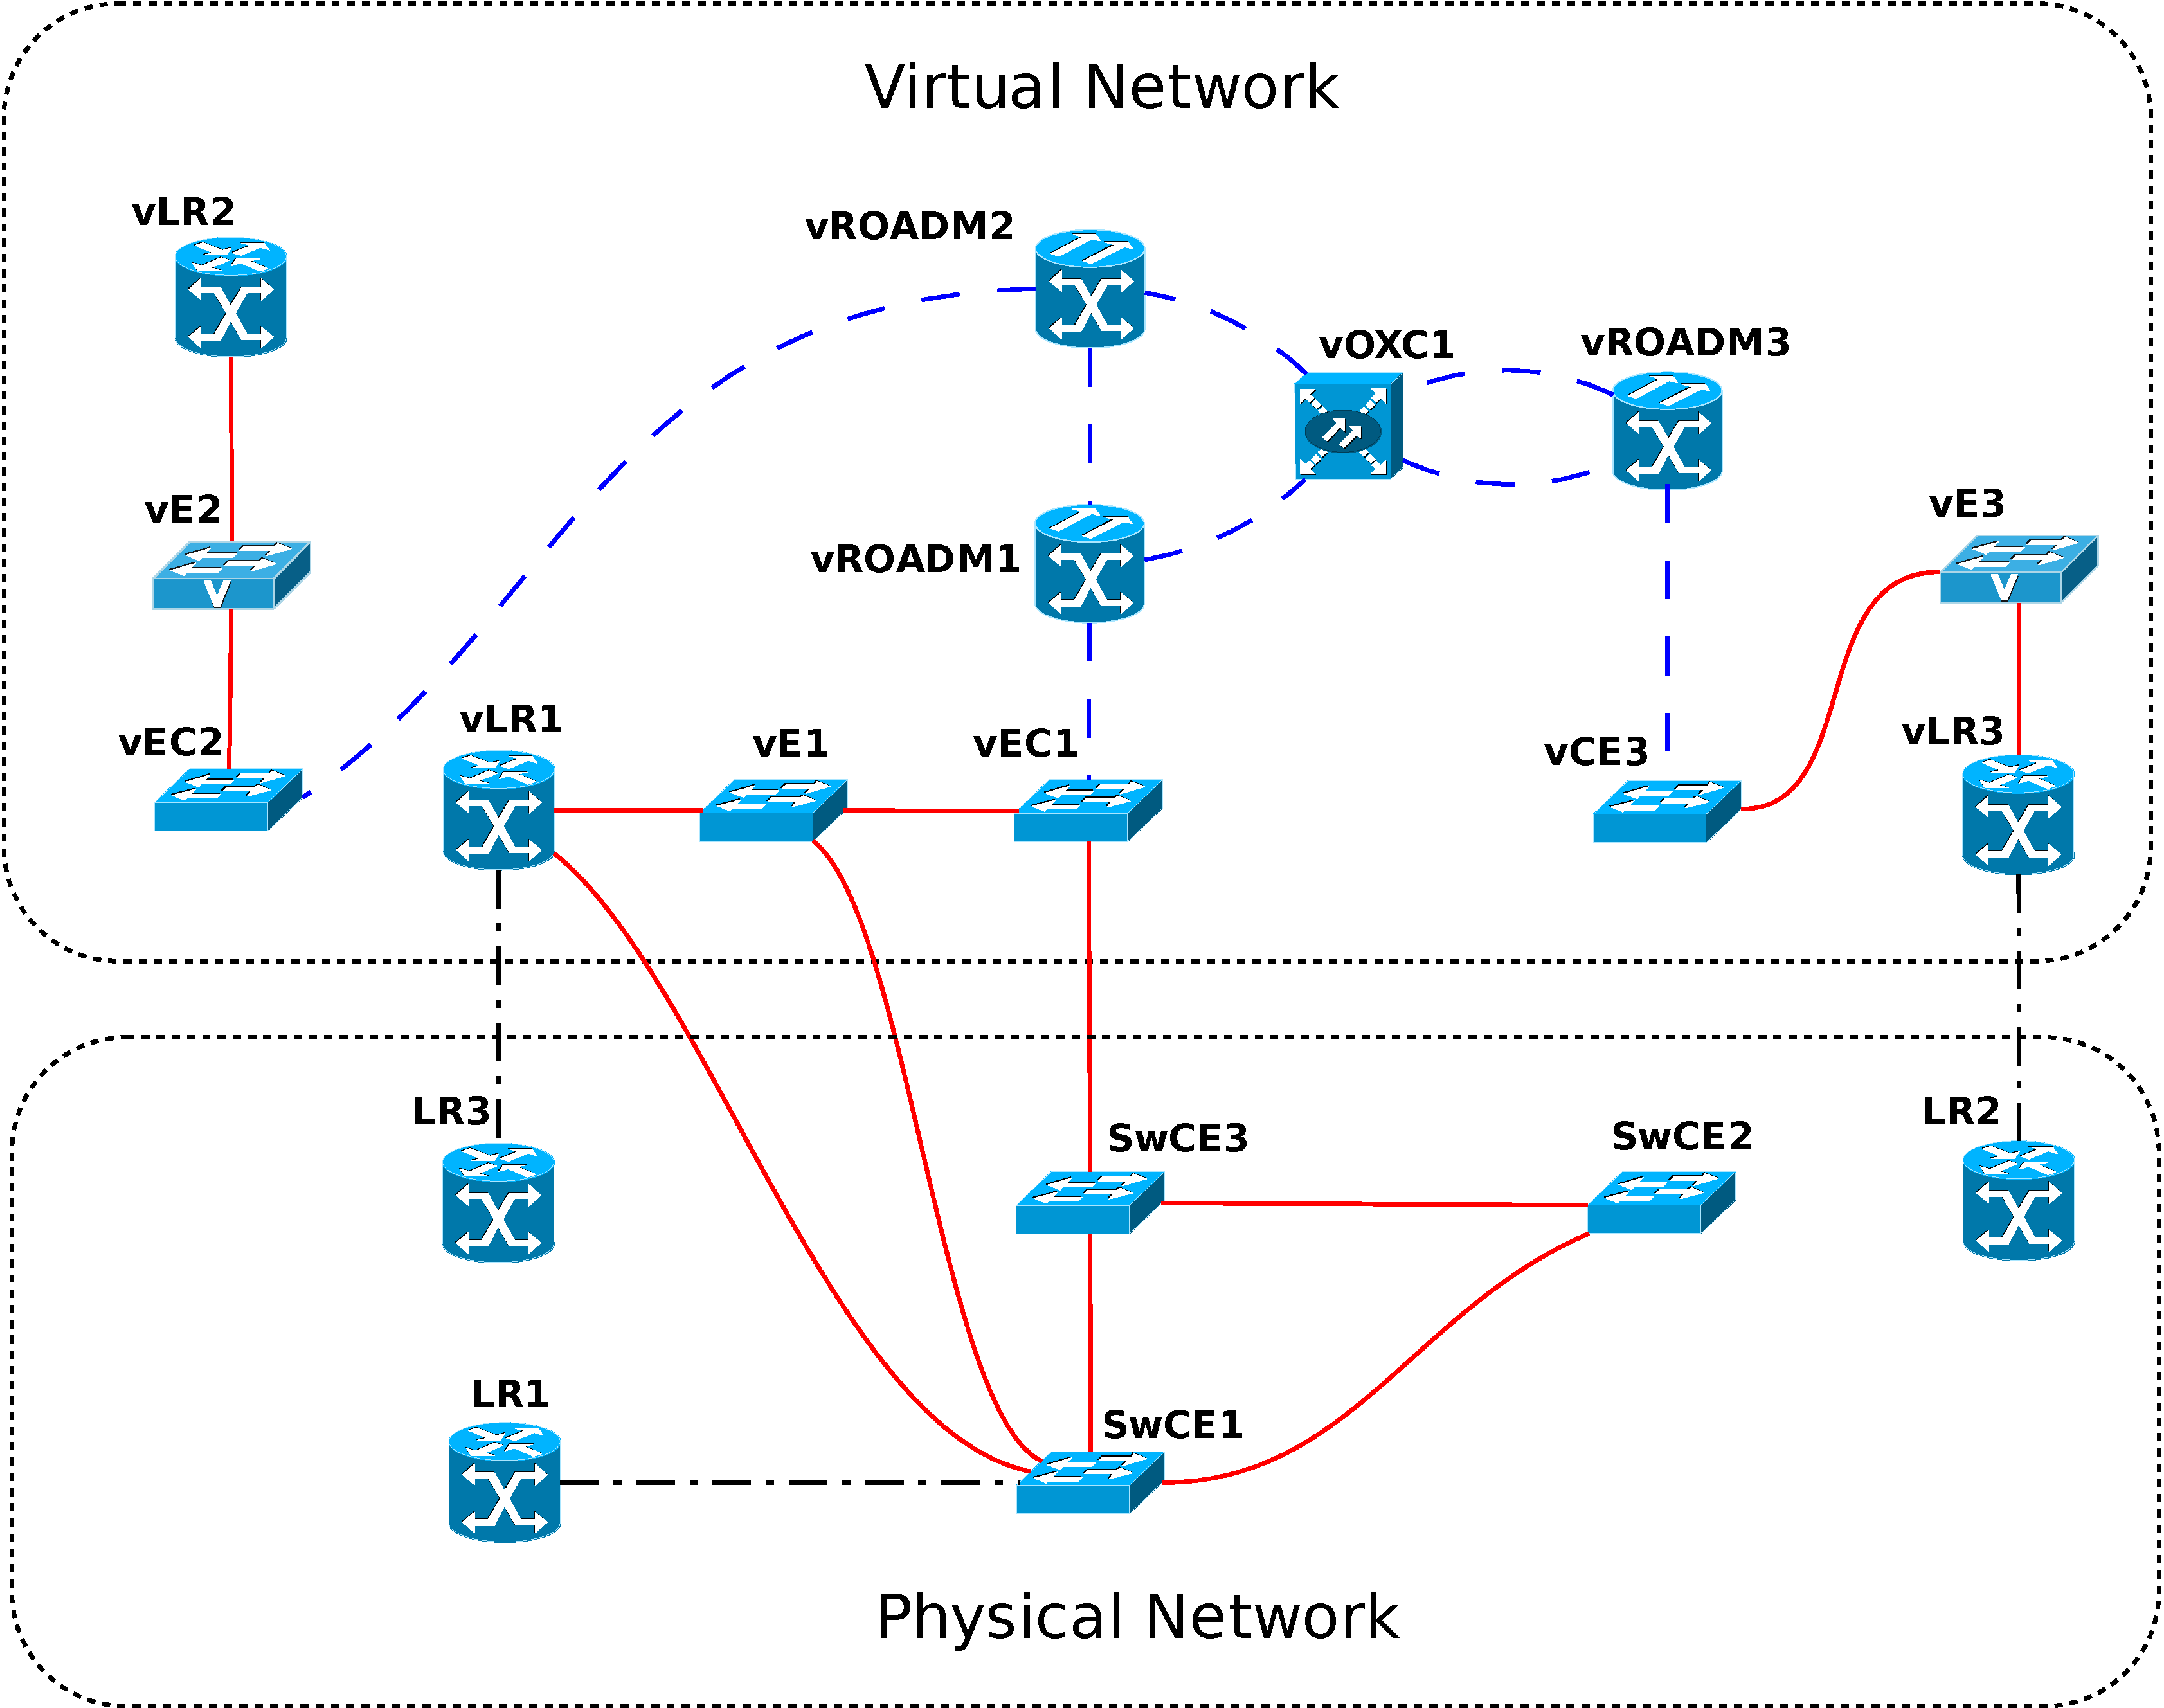
\includegraphics[width=1\textwidth]{img/testbed_model}
    \caption[Testbed representation]{The testbed network.}
    \label{fig:testbed_model}
  \end{center}
\end{figure}

\begin{figure}[!htbp]
  \begin{center}
    \begin{tabular}{|l|l|l|l|}
      \hline
      Node & Type & Description & ID \\ \hline
      vEC1 & Virtual & Ethernet/Optical border & 172.16.100.230 \\
      vEC2 & Virtual & Ethernet/Optical border & 172.16.100.231 \\
      vEC3 & Virtual & Ethernet/Optical border & 172.16.100.232 \\
      vROADM1 & Virtual & Optical Add-Drop Mux & 172.16.100.233 \\
      vROADM2 & Virtual & Optical Add-Drop Mux & 172.16.100.234 \\
      vROADM3 & Virtual & Optical Add-Drop Mux & 172.16.100.235 \\
      vOXC1 & Virtual & Optical Cross-connect & 172.16.100.236 \\
      vE1 & Virtual & Ethernet & 172.16.100.243 \\
      vE2 & Virtual & Ethernet & 172.16.100.244 \\
      vE3 & Virtual & Ethernet & 172.16.100.245 \\
      vLR1 & Virtual & Linux IP/MPLS & 172.16.100.251 \\
      vLR2 & Virtual & Linux IP/MPLS & 172.16.100.252 \\
      vLR3 & Virtual & Linux IP/MPLS & 172.16.100.253 \\
      LR1 & Physical & Linux IP/MPLS & 172.16.100.248 \\
      LR2 & Physical & Linux IP/MPLS & 172.16.100.249 \\
      LR3 & Physical & Linux IP/MPLS & 172.16.100.250 \\
      SwCE1 & Physical & Switchcore Ethernet & 172.16.100.240 \\
      SwCE2 & Physical & Switchcore Ethernet & 172.16.100.241 \\
      SwCE3 & Physical & Switchcore Ethernet & 172.16.100.242 \\
      \hline
    \end{tabular}
    \caption[Testbed network nodes]{Testbed network nodes reference:
      name, type, description and identifier.}
    \label{fig:testbed_legend}
  \end{center}
\end{figure}

\end{document}

%%% Local Variables: 
%%% mode: latex
%%% TeX-master: t
%%% compile-command: "latexmk -pdf ju_liu_thesis"
%%% End:
